\subsection{Einregeln der optimalen Verzögerungszeit}
Da die Leitungen von den SEV zur Koinzidenzschaltung nicht zwingend gleich schnell sind, wird die Verzögerung zwischen den beiden Seiten optimiert.
Die Verzögerungszeit kann in beiden Leitungen separat erhöht werden, indem Kabel mit definierten Verzögerungen zugeschaltet werden.
Eine Verzögerung bei der einen Kabelleitung bewirkt eine relative 'Beschleunigung' der anderen Kabelleitung.
Die Zählrate $N$ wird in Abhängigkeit verschiedener Verzögerungszeiten $T_{\text{VZ}}$ gemessen (Tabelle \ref{tab:verzögerung}, Abbildung \ref{fig:verzögerung}).
\input{tabelleverzögerung.tex}
\begin{figure}[h!]
  \centering
  \includegraphics[width=\textwidth]{figverzögerung.pdf}
  \caption{Optimierung der Verzögerungszeit: Verzögerungszeit $T_{\text{VZ}}$ gegen Spannungsimpuls $U$}
  \label{fig:verzögerung}
\end{figure}
Es wird eine Ausgleichsrechnung der Form
\begin{equation*}
  N = -a \left( T_{\text{VZ}} +b \right)^4+c
\end{equation*}
mit Python \textbf{HIER NOCH DIE VERSION ETC} vorgenommen.
Die Parameter ergeben sich zu
\begin{align*}
  a &=& \SI{4.82149138 \pm 0.236142743e-40}{\frac{1}{s^5}}\\
  b &=& \SI{2.08543593 \pm 0.229205656e-09}{s}\\
  c &=& \SI{208.001211 \pm 3.50366199}{\frac{1}{s}}.\\
\end{align*}
Dabei beschreibt $b$ die seitliche Verschiebung des Maximums und damit den Wert, der fortan als Verzögerung der Leitung gewählt wird.
Damit sind die Signale aus den SEV annähernd gleichzeitig an der Koinzidenzschaltung.
\FloatBarrier
\subsection{Kalibrierung des Multi-Channel-Analysers}
Um vom Channel des Multi-Channel-Analysers auf die zugehörige Zeit zwischen den Impulsen schließen zu können, wird der Multi-Channel-Analyser kalibriert.
Die Channel werden in Abhängigkeit ... vom Doppelimpulsgenerator gegebenen 
\begin{table}[h!]
  \centering
  \caption{Messdaten zu Kalibrierung des Multi-Channel-Analysers}
  \label{tab:kalibrierung}
  \begin{tabular}{c c c c}
    \toprule
%    \multicolumn{3}{c}{$f_{\text{1, theo}}=\SI{0.1}{m}$} & \multicolumn{3}{c}{$f_{\text{2, theo}}=\SI{0.05}{m}$}\\
      Channel & $\Delta$ t $/ 10^{-6} s$ & Channel & $\Delta$ t $/ 10^{-6} s$ \\
      \midrule
         24   &   1407  &  247   &   1680 \\
         46   &   1561  &  270   &   1555 \\
         69   &   1400  &  292   &   1608 \\
         91   &   1294  &  315   &   1384 \\
        113   &   1298  &  337   &   1952 \\
        136   &   1034  &  359   &   1880 \\
        158   &   1502  &  382   &   2008 \\
        180   &   1336  &  404   &   2088 \\
        203   &   1700  &  427   &   2024 \\
        225   &   1644  &  445   &   3384 \\
    \bottomrule
  \end{tabular}
\end{table}

%\end{landscape}
%\end{document}

\begin{figure}[h!]
  \centering
  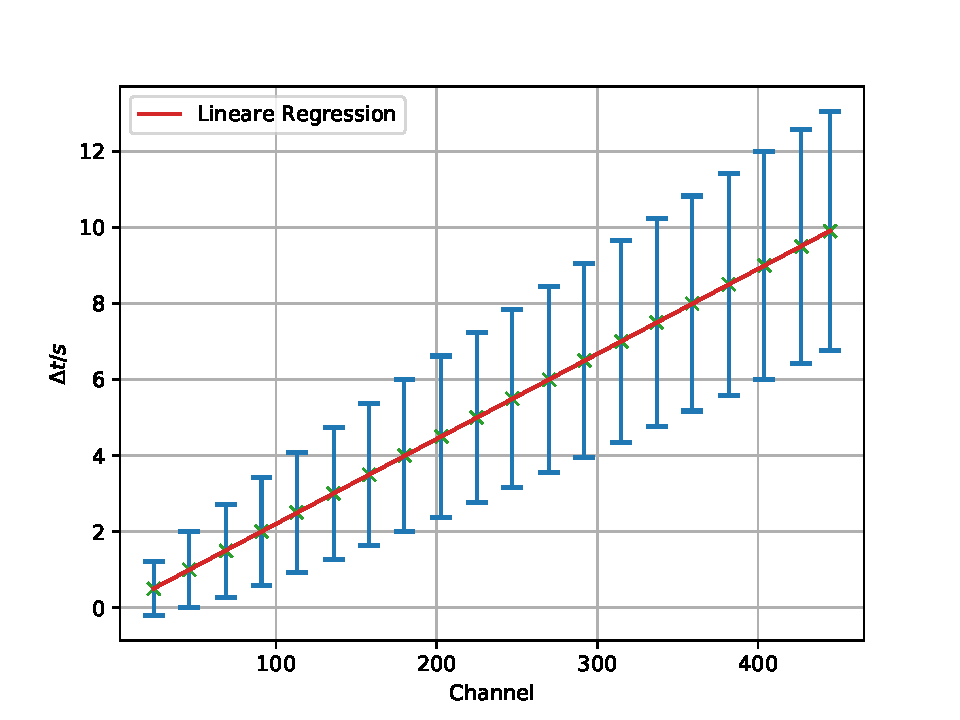
\includegraphics[width=\textwidth]{figkalibrierung.pdf}
  \caption{Kalibrierung des Multi-Channel-Analysers: Zeitlicher Abstand des Doppelimpulses $\Delta$ t gegen den zugehörigen Channel}
  \label{fig:kalibrierung}
\end{figure}
Fit: C $\widehat{=}$ Channel
\begin{equation*}
\Delta t = a \cdot C + b
\end{equation*}
Fitparameter:
\begin{align*}
a  &=&  \SI{ 0.02234091 \pm 1.28401231692e-05}{\frac{1}{s}}  \\
b  &=&  \SI{-0.03080493 \pm 0.00345318109864 }{}  \\
\end{align*}

\FloatBarrier

\subsection{Messung der Lebensdauer}
\begin{figure}[h!]
  \centering
  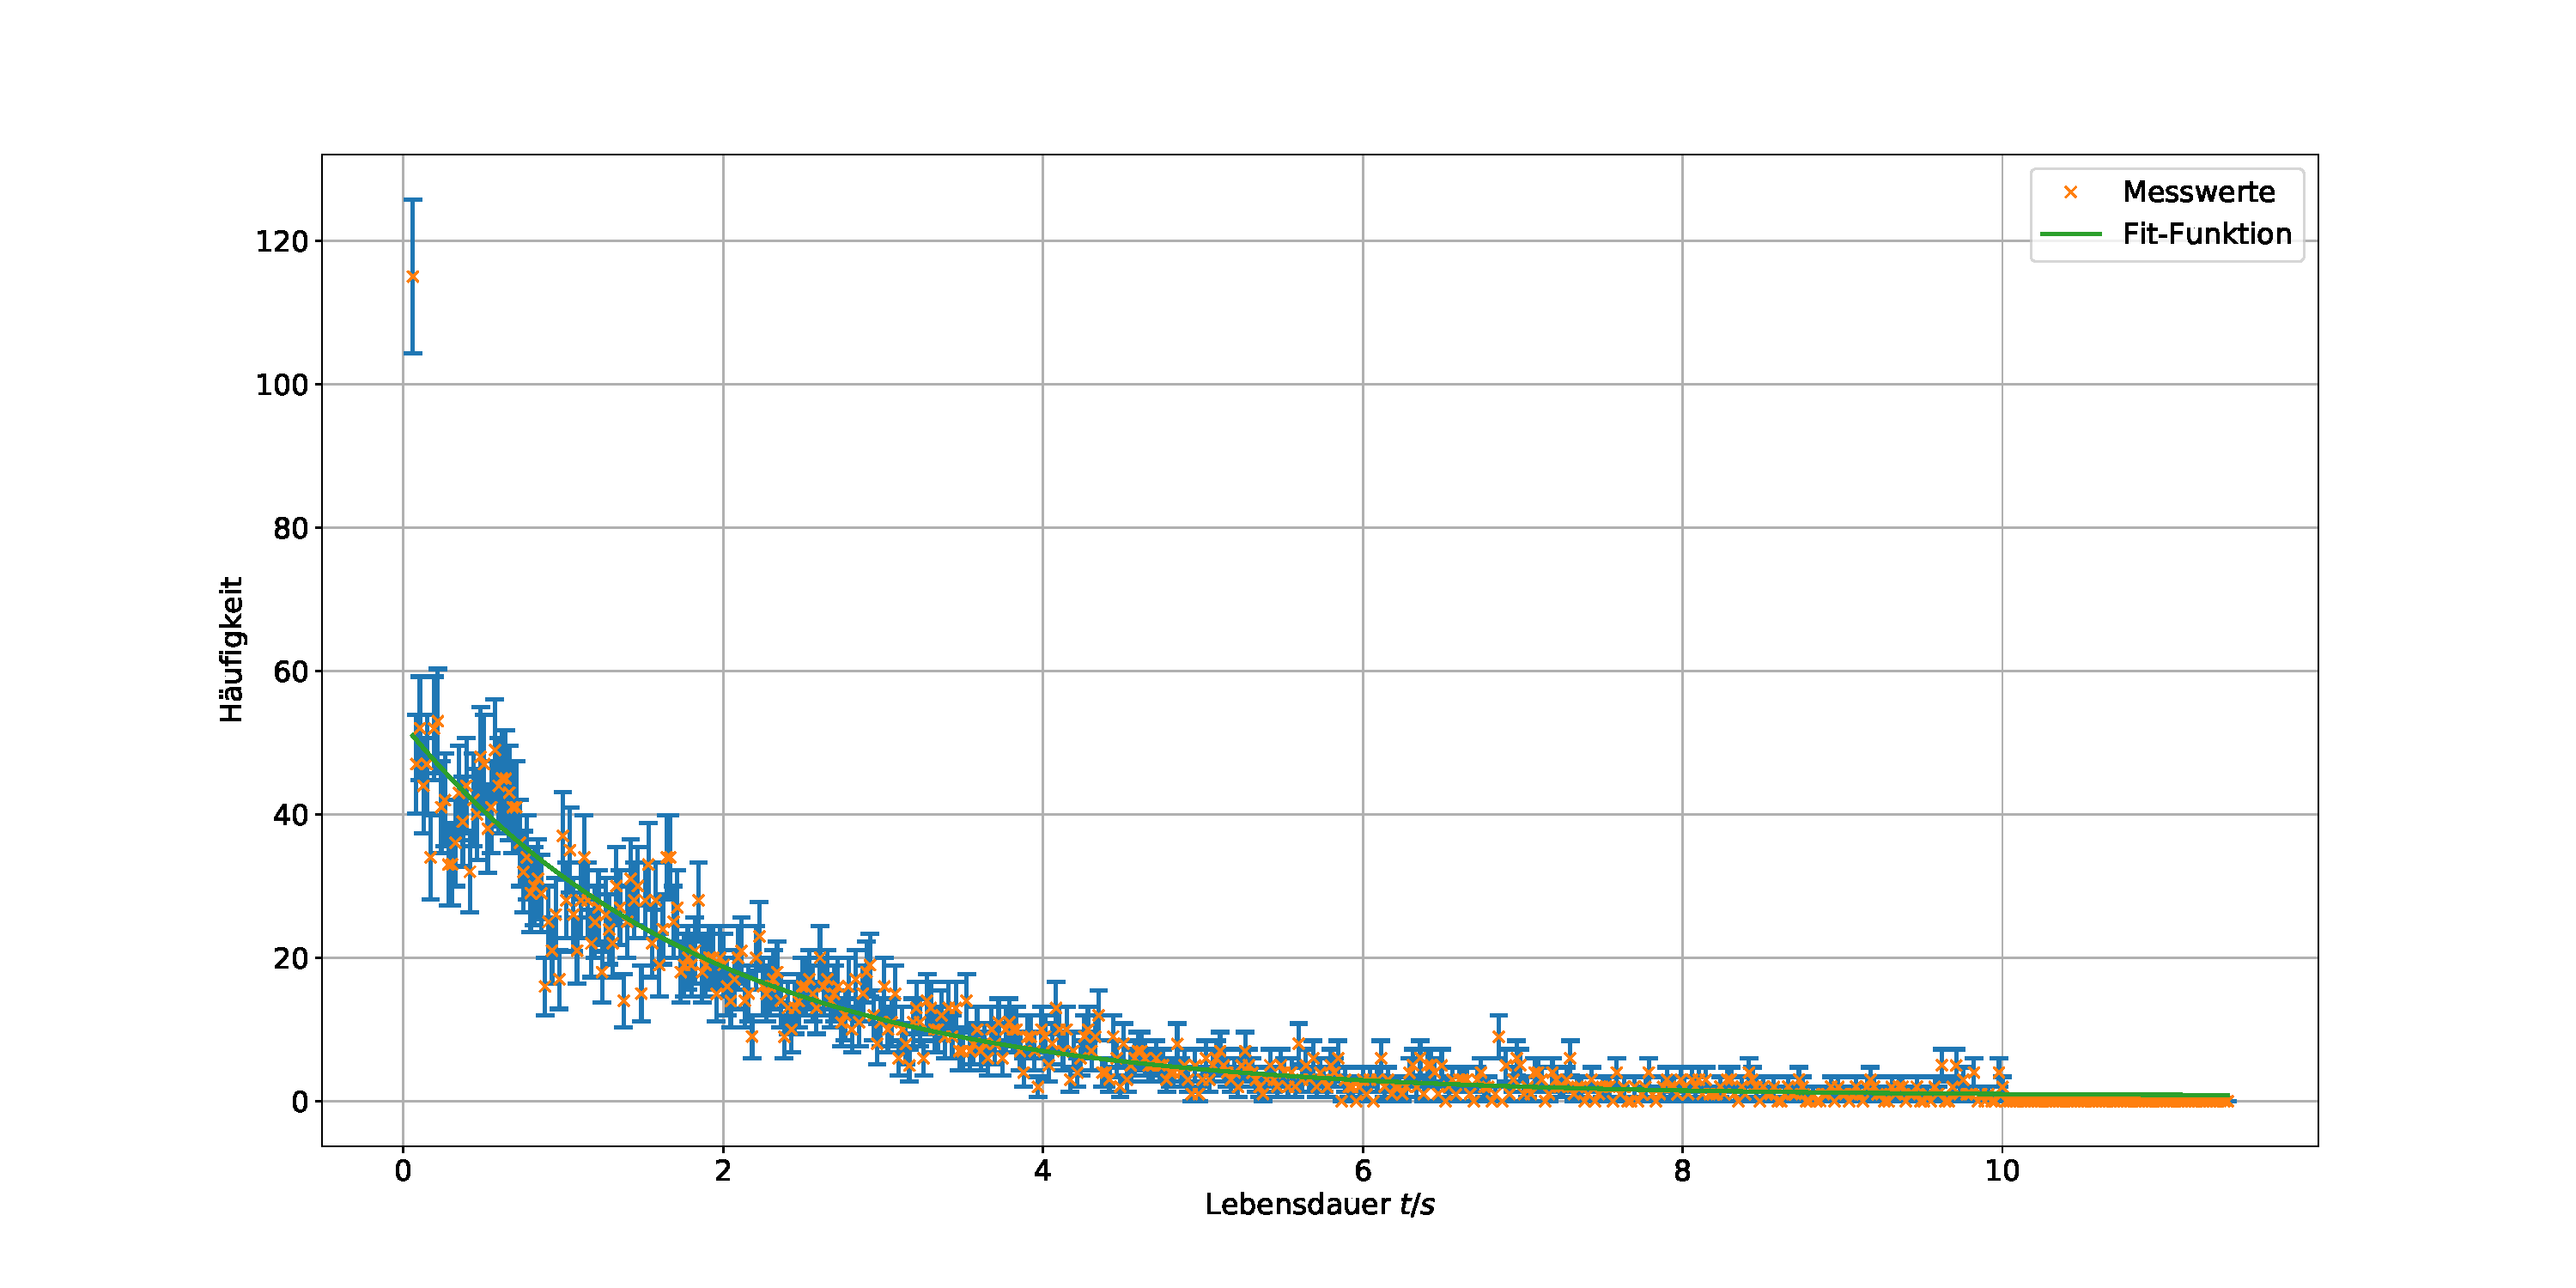
\includegraphics[width=\textwidth]{figmyonen.pdf}
  \caption{Häufigkeit der Myonenzerfälle in Abhängigkeit ihrer Lebensdauer}
  \label{fig:myonen}
\end{figure}
Fit
\begin{equation*}
y = a \exp{(-x b)}+c
\end{equation*}
Fitparameter
\begin{align*}
a  &=&  \SI{51.81005345 \pm 0.9677403}{}\\
b  &=&  \SI{0.52824244 \pm 0.01864355}{}\\
c  &=&  \SI{0.74055349 \pm 0.31446226}{}\\
\end{align*}
\FloatBarrier
